\documentclass[12pt]{article}
\usepackage{geometry}                % See geometry.pdf to learn the layout options. There are lots.
\geometry{letterpaper}                   % ... or a4paper or a5paper or ... 
%\geometry{landscape}                % Activate for for rotated page geometry
\usepackage[parfill]{parskip}    % Activate to begin paragraphs with an empty line rather than an indent
\usepackage{daves,fancyhdr,natbib,graphicx,dcolumn,amsmath,lastpage,url}
\usepackage{amsmath,amssymb,epstopdf,longtable}
\usepackage{paralist} 
\DeclareGraphicsRule{.tif}{png}{.png}{`convert #1 `dirname #1`/`basename #1 .tif`.png}
\pagestyle{fancy}
\lhead{CE 3372 -- Water Systems Design}
\rhead{FALL 2017}
\lfoot{EXERCISE 8}
\cfoot{}
\rfoot{Page \thepage\ of \pageref{LastPage}}
\renewcommand\headrulewidth{0pt}

\begin{document}
\begin{center}
\textbf{MEMORANDUM}
%{\textbf{{ CE 3372 -- Water Systems Design} \\ {Exercise Set 2}}}
\end{center}
\begingroup
\begin{tabular}{p{1in} p{5in}}
To: & P. N Guin \\ ~\\
From: & P. Olar Bear \\ ~\\
Date: & 04MAR2024 \\ ~\\
Subject: & CE 3372 -- Water Systems Design, Exercise Set 8. ~\\


\end{tabular}
\endgroup
\section*{\small{Purpose}}  
This memorandum presents the estimation of demand for a subdivision and a simple network analysis using EPANET for the network in ES7 (the prior exercise set).  
The results for each problem are presented in the narrative below.
\section*{\small{Problem 1 Solution:}}
Figure \ref{fig:newport-pipe-layout} is the skeletonized layout for an EPANET model of the water distribution system for a proposed executive home subdivision.  
The figure depicts a supply reservoir, a pump, a check valve, pipes, and demand nodes.  
The system is a hybrid branch-loop system; the branches are relatively short.

\begin{figure}[h!] %  figure placement: here, top, bottom, or page
\centering
   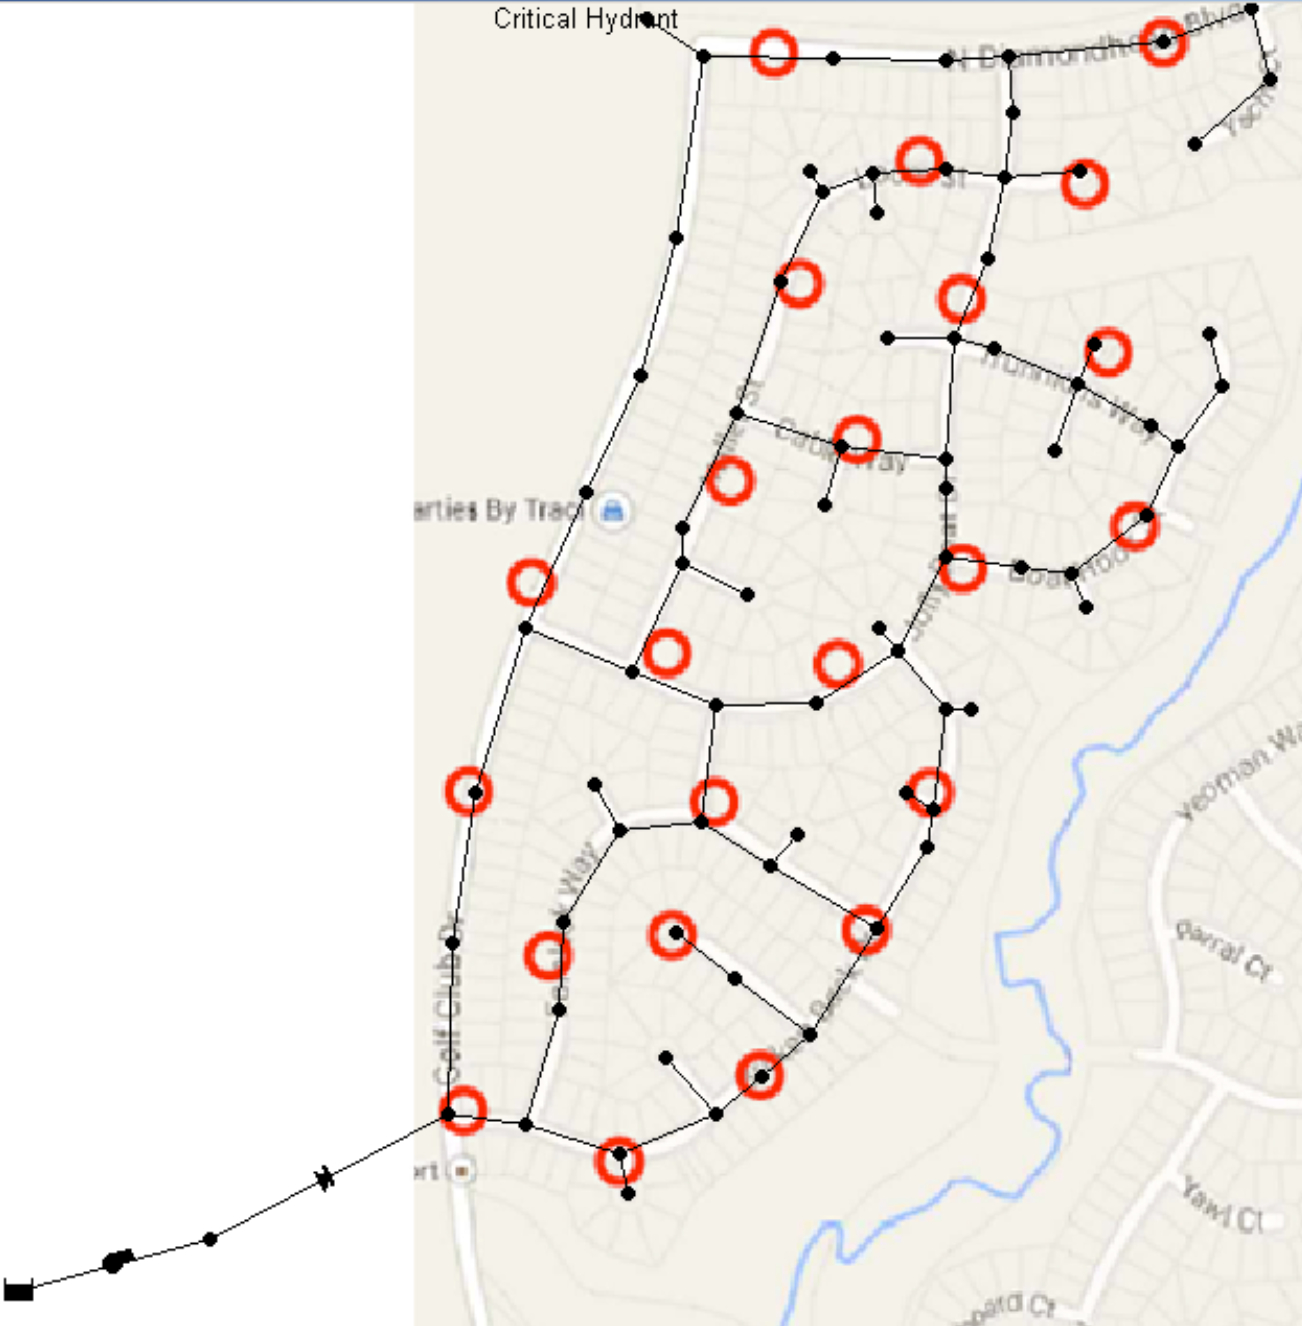
\includegraphics[width=6in]{newport-pipe-layout.jpg}
   \caption{Newport Subdivision EPANET Model Pipe Layout}
   \label{fig:newport-pipe-layout} 
\end{figure}

Demand is estimated by counting the number of lots depicted on the map, then determining the type of structure on each lot, and finally determining the occupancy per structure (or lot).  Once the total occupancy is estimated the product of that count and an average daily demand establishes the demand for the water distribution system. 

The approximate count of lots depicted on Figure \ref{fig:newport-pipe-layout} is 409.  
Each lot is to house an executive home, with an average occupancy of 4 persons.  
A typical demand for a person is 100 gallons per day.\footnote{Value from \url{http://water.usgs.gov/edu/qa-home-percapita.html} accessed 12 Oct 2016}, however because these are executive homes, there are likely pools, spas, and semi-exotic gardens so the demand is likely higher.  
As an estimate the demand range is 100 to 200 gpd per person. \\~\\
Using these values, the total daily demand is $409 \text{~lots} \times 4 \text{~persons per lot} \times 100 \text{~gpd per person} = 122,700 \text{~gpd} $ for the low estimate and $ 245,400 \text{~gpd} $ for the high estimate.
\clearpage
%%%%%%%%%%%%%%%%%%%%%%%%%%%%%%%%%%%%%%%%%%%%%%%%%%%%%%%
%%%%%%%%%%%%%%% PROBLEM 2 %%%%%%%%%%%%%%%%%%%%%%%%%%%%%%%%%
%%%%%%%%%%%%%%%%%%%%%%%%%%%%%%%%%%%%%%%%%%%%%%%%%%%%%%%
\section*{\small{Problem 2 Solution:}}
Figure \ref{fig:NetworkLayout} is a screen capture of an EPANET model of a five-pipe network with a water supply source (a reservoir) connected at Node 1, and demands at Nodes 1-5.

\begin{figure}[h!] %  figure placement: here, top, bottom, or page
\centering
   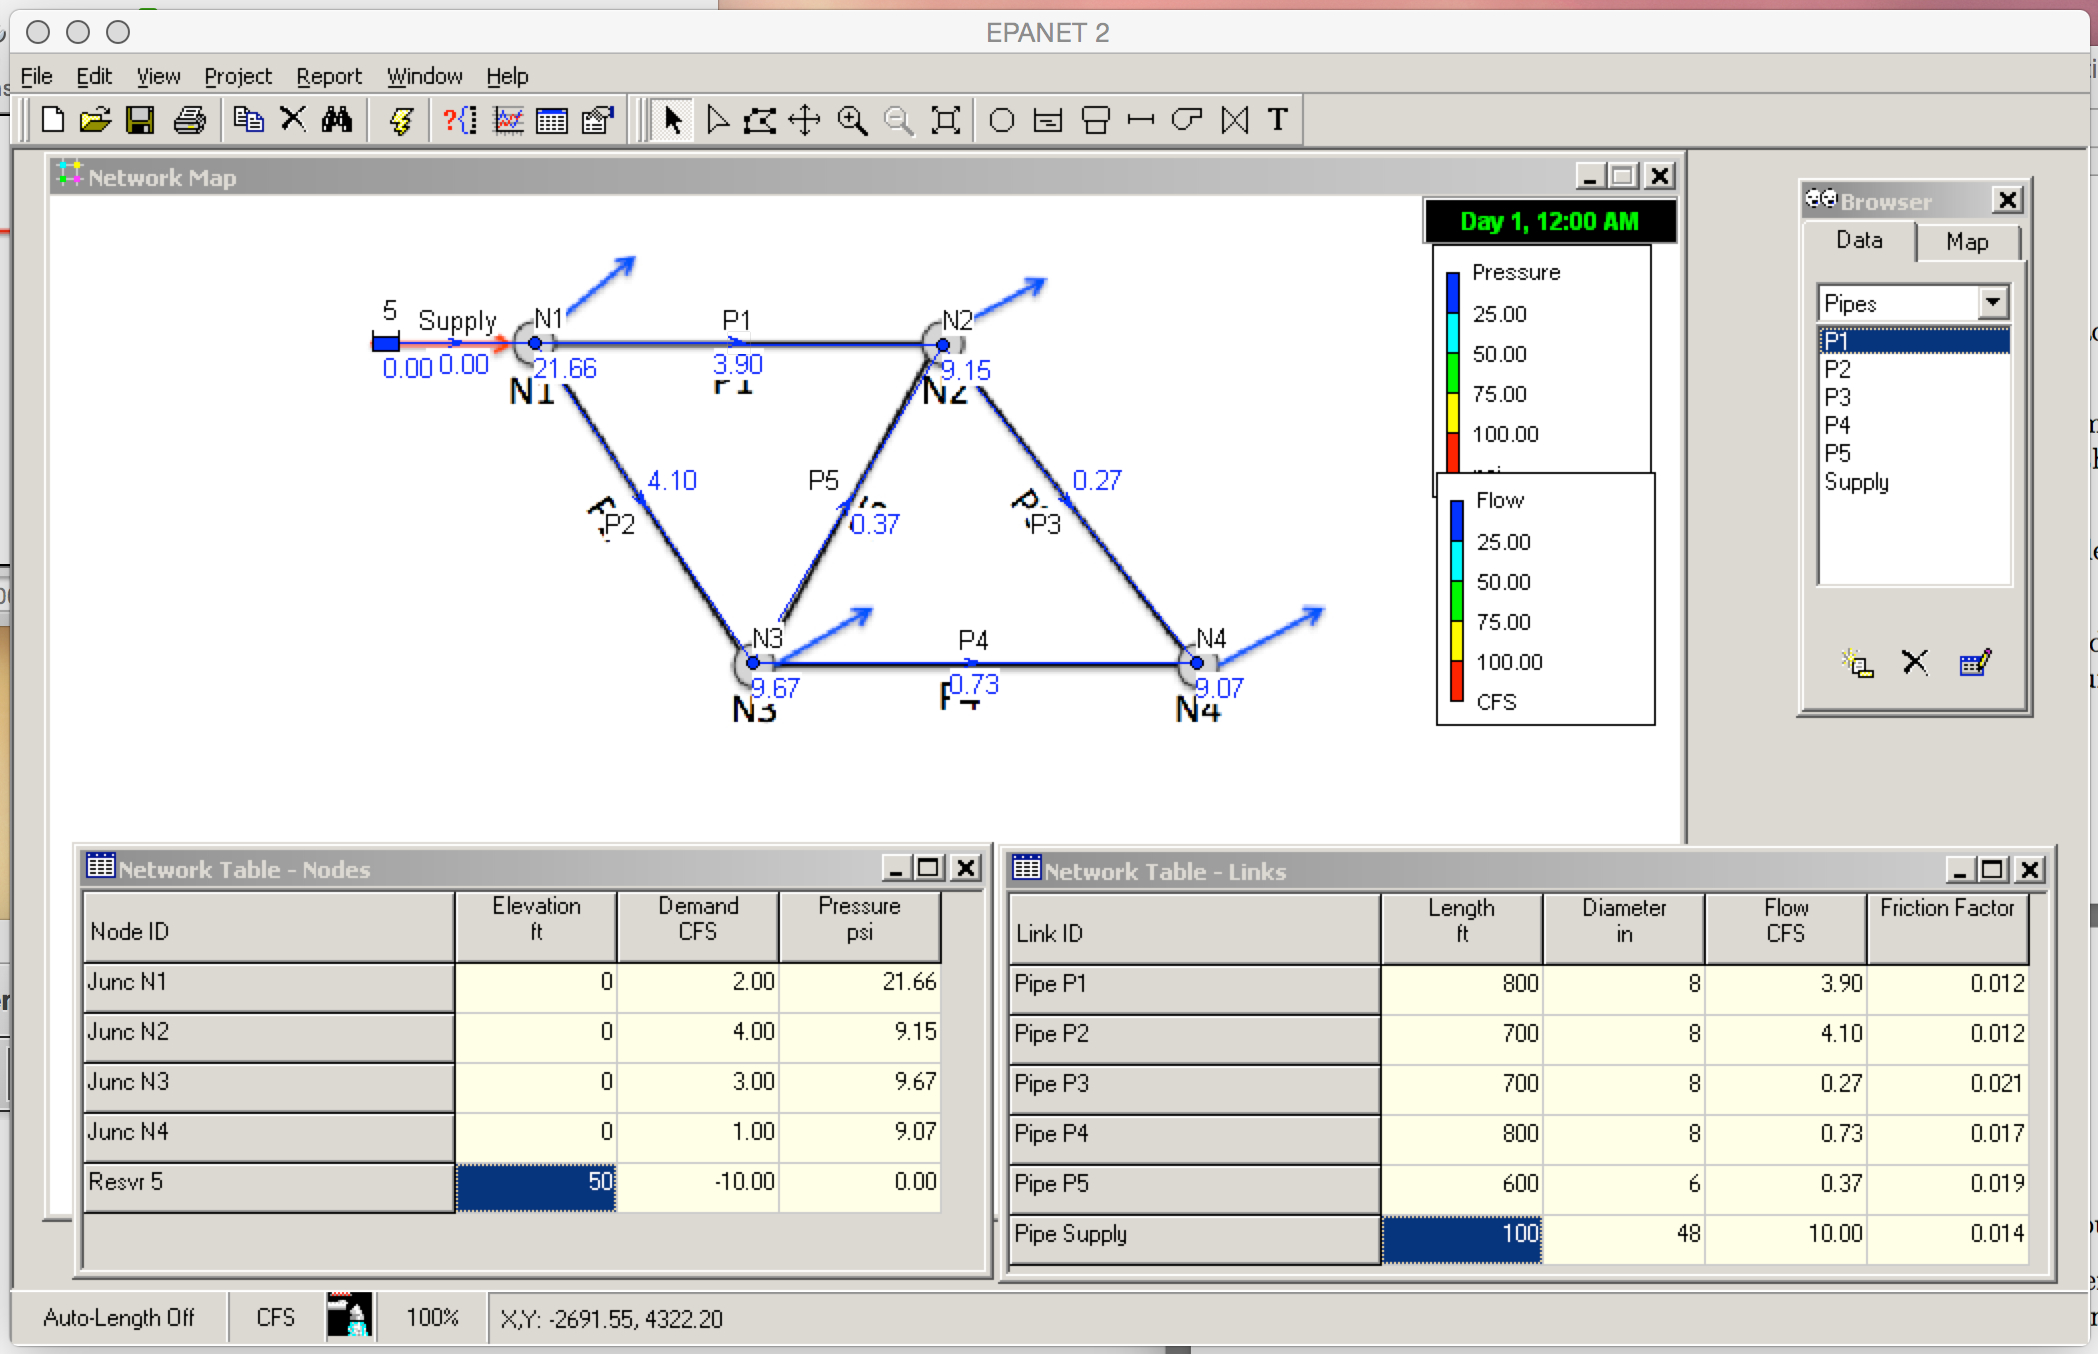
\includegraphics[width=7in]{NetworkSimulation.jpg}
   \caption{Layout of Simple Network}
   \label{fig:NetworkLayout} 
\end{figure}

The screen capture shows the network map, with the Node ID and Node Pressures (in psi) displayed on the map, and with the Pipe ID and Pipe Flow Rates on the map.

The screen capture displays a table (lower left of the image) that lists each node name, node elevation, and the resultant pressure in U.S. Customary units.  The screen capture displays another table (lower right of the image) that lists each pipe name, length, diameter, computed friction factor, and the resultant flow rate in U.S. Customary units.  

The node with the lowest pressure (excluding the reservoir) is node N4 with a reported pressure of 9.07 psi.

The EPANET output report appears as the remainder of this memorandum.

\begin{verbatim}
  Page 1                                           10/12/2016 3:29:15 AM
  **********************************************************************
  *                             E P A N E T                            *
  *                     Hydraulic and Water Quality                    *
  *                     Analysis for Pipe Networks                     *
  *                           Version 2.0                              *
  **********************************************************************
  Input File: 
  Link - Node Table:
  ----------------------------------------------------------------------
  Link           Start          End                Length  Diameter
  ID             Node           Node                   ft        in
  ----------------------------------------------------------------------
  P1             N1             N2                    800         8
  P2             N1             N3                    700         8
  P3             N2             N4                    700         8
  P4             N3             N4                    800         8
  P5             N3             N2                    600         6
  Supply         5              N1                    100        48
  Node Results:
  ----------------------------------------------------------------------
  Node                Demand      Head  Pressure   Quality
  ID                     CFS        ft       psi          
  ----------------------------------------------------------------------
  N1                    2.00     50.00     21.66      0.00
  N2                    4.00     21.13      9.15      0.00
  N3                    3.00     22.32      9.67      0.00
  N4                    1.00     20.93      9.07      0.00
  5                   -10.00     50.00      0.00      0.00 Reservoir
  Link Results:
  ----------------------------------------------------------------------
  Link                  Flow  VelocityUnit Headloss    Status
  ID                     CFS       fps    ft/Kft
  ----------------------------------------------------------------------
  P1                    3.90     11.17     36.09      Open
  P2                    4.10     11.74     39.53      Open
  P3                    0.27      0.76      0.29      Open
  P4                    0.73      2.10      1.75      Open
  P5                    0.37      1.86      2.00      Open
  Supply               10.00      0.80      0.04      Open
\end{verbatim}







\end{document}  